\typeout{NT FILE chapter4.tex}
\chapter{ Modelling Experiments} \label{experiments_chapter}
\paragraph{}
In this chapter, experiments will be performed to identify the best pre-processing and training parameters to increase the classification performance of the model of choice. 
All the below experiments were carried out using this author's personal computer with Intel(R) Core(TM) i7-10750H \gls{CPU} @ 2.60GHz, 16GB \gls{RAM} with a GeForce RTX 2070 with Max-Q Design 8GB \gls{GPU}
\section{Choosing the most appropriate classification model} \label{classification_models}
% \subsection{Scene classification model}
% For the scene classification model Transfer Learning was used with Mobile V2 using ImageNet weights
\subsection{Pixel-wise classification model} \label{pixel_model}
After framing the problem as a scene classification problem and getting quite good results, in the search for a more challenging problem and due to the availability of data labels for each pixel form polygons it was decided by the author to frame the problem as a pixel-wise classification problem.

The decision to use a U-Net architecture as baseline came from a lot of the literature on remote sensing images being modified U-Net architectures, below is a description of the U-Net architecture this project implements as a baseline.
\paragraph{}
In this project a \textbf{convolution block($x$, $z$)} consists of:
    \begin{enumerate}
        \item \textbf{2D convolutional layer with $x$ channels} with 3x3 filter dimensions, stride of 1 and "same" padding so that if you use a stride of 1, the layer's outputs will have the same spatial dimensions as its inputs.
        \item \textbf{Dropout layer with $z$ rate} of input units to drop.
        \item \textbf{2D convolutional layer with $x$ channels} with 3x3 filter dimensions, stride of 1 and "same" padding so that if you use a stride of 1, the layer's outputs will have the same spatial dimensions as its inputs.
        \item \textbf{2D Maximum Pooling layer} with a 2x2 pooling dimension, no padding and stride defaulting to pooling dimensions, this MAx pooling layer is omitted in the layers after the first Transpose convolutional layer.
    \end{enumerate}
\paragraph{}
In this project a \textbf{transpose convolution block($x$)} consists of:
    \begin{enumerate}
        \item \textbf{2D transpose convolutional layer with $x$ channels} with 2x2 filter dimensions, stride of 2x2 and "same" padding.
        \item \textbf{Skip connection} concatenate weights of 2D transpose convolutional layer with $x$ channels and the weights of the previous 2D convolutional layer with the same number of $x$ channels.
    \end{enumerate}    
\paragraph{}
With the above concepts and the U-Net architecture diagram introduced in Figure \ref{fig_unet} in mind, the initial baseline U-Net architecture used in this project is composed of the following blocks in sequential order:
%maybe should make a picture to make this clearer

    \begin{enumerate}
        \item convolution block(16, 0.1), convolution block(32, 0.1), convolution block(64, 0.2), convolution block(128, 0.2)
        \item convolution block(256, 0.3)
        \item transpose convolution block(128), convolution block(128, 0.2), transpose convolution block(64), convolution block(64, 0.2), transpose convolution block(32), convolution block(32, 0.1), transpose convolution block(16), convolution block(16, 0.1)
        \item finally an output layer of a 1x1 2D convolutional layer with a sigmoid activation function to create the per-pixel class probability map
    \end{enumerate}
\subsection{Evaluating the use of transfer learning}
Given the small labelled dataset and the difference compared to ImageNet, since we are dealing with aerial shots of landscapes, the rule of thumb would be to fine-tune the hidden layers.
\paragraph{}
However, given that most models are only trained on a depth of 3 channels, the weights of such pre-trained models are not compatible with the choice of 4 channels or more.
Therefore, this author deemed it better to re-train the model even though there is a small labelled dataset present.
\subsection{Pixel-level class imbalance} \label{class_imbalance}

Given the process of data collection adopted initially in this project where the area of interest i.e. the \gls{RTS} positive pixels are in the centre of the image and an area of $256$x$256$ is "cut" around it to create a patch. 

The large area of the patch created a pixel-wise class imbalance which led to the model's poor performance when identifying positive \gls{RTS} sample. This is due to the low level of \gls{RTS} pixels where $75\%$ of images have less than $360$ pixels this when compared with the area size of a $256$x$256$ image is less than $0.55\%$ of the image, a needle in a haystack as some would say. By for example reducing the image area by $16$ times to $4096$, the area of a $64$x$64$ image that is now more almost $9\%$ of the image.

It also made accuracy a very misleading metric to follow, since the model would be rewarded for the hundreds of negative sample pixels it correctly identified, but wouldn't absorb the cost of misclassifying the pixels this project is most interested in finding the \gls{RTS} pixels. 

For example, say that $1\%$ of the image is made up of positive \gls{RTS} pixels while the rest is made up of background negative pixels, if the model predicts negative background pixel for the whole image it would still be $99\%$ accurate, even though it didn't classify a single \gls{RTS} pixel correctly, this can be very misleading.
This unsuitability of accuracy as a performance measure, is also part of the justification for using the dice score introduced in section \ref{performance_measures} as the performance measure of choice in the experiments that follow. Being the harmonic mean between precision and recall, it makes it one of the best candidates for unbalanced class problems.

Following this realisation, the size of the input patch was reduced to create a more even pixel-wise class distribution, the results of this experiment will be described in detail in section \ref{patch_size_exp}.

\subsection{Experiment set up}
\paragraph{}
In order to identify a baseline model, trial runs for only 20 epochs were performed in a grid search methodology to identify a suitable baseline model to use in the following experiment sections. After evaluating the dice coefficient, the parameters of the baseline model are:

\begin{center}
    \begin{tabular}{c|c}     
    \textbf{Parameter} & \textbf{Value}  \\
    \hline
    Patch Size
    &  64x64 \\
    \hline
    Normalisation
    & na\"ive \\
    \hline
    Augmentation Method
    &  None \\
    \hline
    Activation Function
    &  Exponential Linear Unit (ELU) \\
    \hline
    Loss Function
    &  CE Dice Loss\\
    \hline
    Optimiser
    &  Adam \\
    \hline
    Batch size
    &  $4$ \\
    \hline
    Initial Learning Rate
    &  $0.0001$  \\
    \hline
    Learning Rate Schedule
    &  ReduceLROnPlateau  \\
    \hline
    Initialisation method
    &  "He" Normal  \\
    \hline
    Regulariser
    &  Dropout with varying rates \\
    \end{tabular}
\end{center}

For each of the experiments, there will be trial runs of each potential value for $50$ epochs to identify the best value, keeping everything else as the baseline value. The objective is to maximise the performance measure of choice, the dice coefficient (coef) by minimising the loss.
\section{Preprocessing experiments}
The experiments in this section ran for $50$ epochs, due to the non-deterministic nature of neural networks the results are not always of comparable performance between experiments, but were run within the same Tensorflow session within each experiment for comparability.
\subsection{Size of the input patch} \label{patch_size_exp}
As described in section \ref{class_imbalance}, class imbalance became an issue with model performance, in order to test if cropping the image to create a more balanced pixel-level class distribution could be linked to model performance, experiments were carried out. This was done by cropping the input patch from $256$×$256$ to $128$×$128$, $64$×$64$ and finally $32$×$32$ pixels, which would be reflected in the input layer dimensions of the model as well.

\begin{figure}[hbt!]
    \centering
    % \begin{minipage}[c]{0.45\linewidth}
    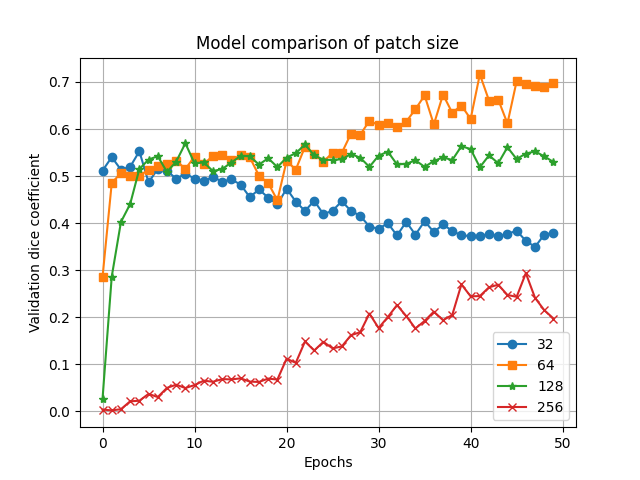
\includegraphics[width=0.75\linewidth]{patch size_Validation dice coefficient.png}
    \caption{Input patch size Dice Coefficient comparison}
    \label{patch_dice}
    %     \end{minipage}
    %     \hfill
    %     \begin{minipage}[c]{0.45\linewidth}
    %     \includegraphics[width=\linewidth]{patch_size_evaluation_loss.png}
    %     \caption{Input patch size loss comparison}
    %     \label{patch_loss}
    % \end{minipage}
\end{figure}
\paragraph{}
% As seen from Figure \ref{patch_dice}, 
The model with the highest validation dice coefficient was the one where the image was cropped to a $64$×$64$ pixel area, with a validation dice coefficient of $0.7$ vastly outperforming the other patch sizes, shown in figure \ref{patch_dice}.
\begin{table}[ht!] 
    \begin{center}
    \begin{tabular}{ccccccc} 
    \toprule
       & \multicolumn{3}{c}{Dice Coefficient}     & \multicolumn{3}{c}{Loss} \\
    Patch size & Validation & Training & Test & Validation    & Training    & Test   \\ \midrule
32 & 0.38 & 0.59 & 0.34 & 1.2 & 0.82 & 1.27 \\ \rowcolor{lightgray} 64 & 0.7 & 0.82 & 0.78 & 0.5 & 0.26 & 0.3  \\ 128 & 0.53 & 0.6 & 0.62 & 0.57 & 0.48 & 0.43  \\ 256 & 0.2 & 0.31 & 0.14 & 0.84 & 0.72 & 0.9  \\
\bottomrule
    \end{tabular}
  \end{center} 
  \caption{Input patch size comparison of Dice Coefficient and Loss}\label{tab_patch}
\end{table}
\paragraph{}
The results shown in table \ref{tab_patch}, indicate increasing performance with the decrease of the patch size, up until the 64×64 patch size, which would indicate that at 32×32 patch size the context surrounding the larger thaw slumps (which just fit in the 64×64 patch) is lost leading to decreasing performance, therefore the remaining experiments of this project will use a 64×64 patch size and input layer dimensions.
\subsection{Normalisation of input}
\paragraph{}
Another key factor in the success of the training of the model is adequate normalisation of the inputs, specially with the extremely high values reflectance values in remote sensing images can take, as described in section \ref{img_norm}. Getting this wrong can lead to explosive gradients and invalid (NaN) loss and performance metrics when training the model, as witnessed in this project.

The na\"ive approach of simply converting any pixel $x>10,000=10,000$ followed by $x=x/10,000$ was the one used for the initial experiments.

In order to implement the other two transformations $[0,1]$ interval and z-score, introduced in detail in section \ref{img_norm}, the maximum, mean and standard deviation of all $64$×$64$ training set images were calculated across each band/channel independently. This is done using only the training set images to prevent the distribution of the validation and test set leaking into the model.
\begin{figure}[hbt!]
    \centering
    % \begin{minipage}[c]{0.45\linewidth}
    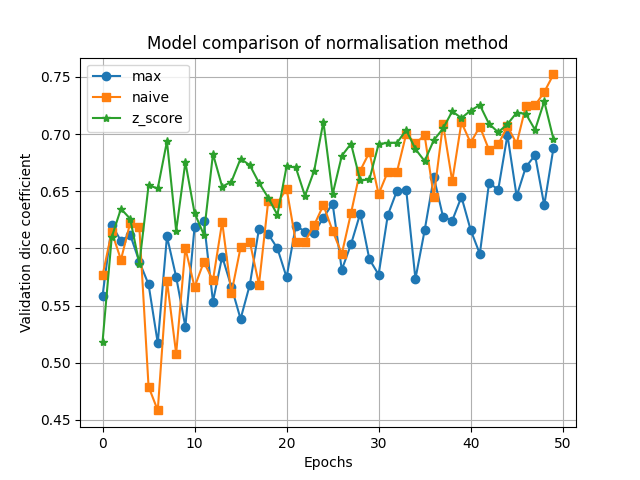
\includegraphics[width=0.75 \textwidth]{normalisation method_Validation dice coefficient.png}
    \caption{Normalisation method Dice Coefficient comparision}
    \label{norm_dice}
    % \end{minipage}
    %     \hfill
    %     \begin{minipage}[c]{0.45\linewidth}
    %     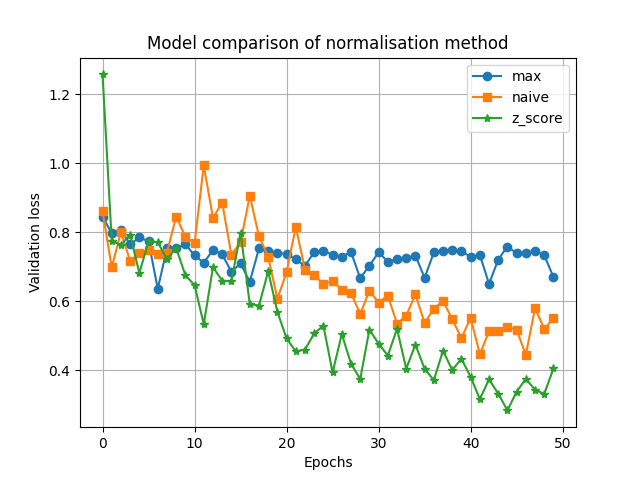
\includegraphics[width=\linewidth]{normalisation method_Validation loss.png}
    %     \caption{Normalisation method loss}
    %     \label{norm_loss}
    % \end{minipage}
\end{figure}

Given the better performance of the  na\"ive normalisation method seen in Figure \ref{norm_dice}, it will be used for the rest of the experiments here onward.
\begin{table}[ht!] 
    \begin{center}
    \begin{tabular}{ccccccc} 
    \toprule
       & \multicolumn{3}{c}{Dice Coefficient}     & \multicolumn{3}{c}{Loss} \\
    Normalisation method & Validation & Training & Test & Validation    & Training    & Test   \\ \midrule
    % max & 0.53 & 0.58 & 0.45 & 0.67 & 0.62 & 0.78  \\ naive & 0.68 & 0.86 & 0.82 & 0.55 & 0.21 & 0.27  \\ \rowcolor{lightgray} z-score & 0.77 & 0.87 & 0.87 & 0.41 & 0.18 & 0.18  \\
    max & 0.69 & 0.87 & 0.71 & 0.49 & 0.18 & 0.41  \\ \rowcolor{lightgray} naive & 0.75 & 0.89 & 0.8 & 0.39 & 0.16 & 0.27  \\ z score & 0.7 & 0.92 & 0.8 & 0.5 & 0.13 & 0.28  \\

    \bottomrule
    \end{tabular}
  \end{center} 
  \caption{Normalisation method comparison of Dice Coefficient and Loss}\label{tab_norm}
\end{table}
\subsection{Data Augmentation}
\paragraph{}
Data Augmentation can be invaluable when the dataset is small, and even more when the data collection is biased. The main purpose of data augmentation in this project is to correct the bias of \gls{RTS} positive pixels always being in the centre of the image.

In that sense, the most useful data augmentation transformation is translation or shift, where the image is translated to the right or left according to certain parameter. The implementation of this was done in the \gls{NN} itself has one of the initial layers with Keras's “RandomTranslation” layer. One layer with an output shifted vertically and horizontal by a random amount of $20\%$ in each direction, to fill the pixels left blank by this translation the fill mode of choice was bipolar interpolation of the nearest pixels.

At this stage a rotation augmentation method was also implemented for comparison, in the same way with the same parameter settings but using Keras's “RandomRotation” layer instead, which rotates the image clockwise or anti-clockwise instead by the random amount of $20\%$, with the same fill method. 

The experiment results can be seen in Figures \ref{aug_dice}, no augmentation (baseline) yields better results than rotation, translation, or both implementations at once.

This could be due to changes in the geometry or lighting causing the \gls{ROI} or important contextual background pixels in the image to lose the original features that helped identify the \gls{RTS} pixels correctly.

\begin{figure}[hbt!]
    % \begin{minipage}[c]{0.45\linewidth}
    \centering
    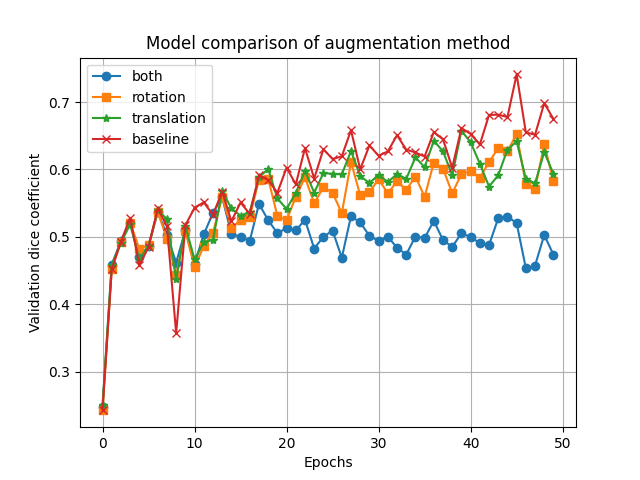
\includegraphics[width=0.75 \textwidth]{augmentation method_Validation dice coefficient.png}
    \caption{Augmentation method Dice Coefficient comparison}
    \label{aug_dice}
    %     \end{minipage}
    %     \hfill
    %     \begin{minipage}[c]{0.45\linewidth}
    %     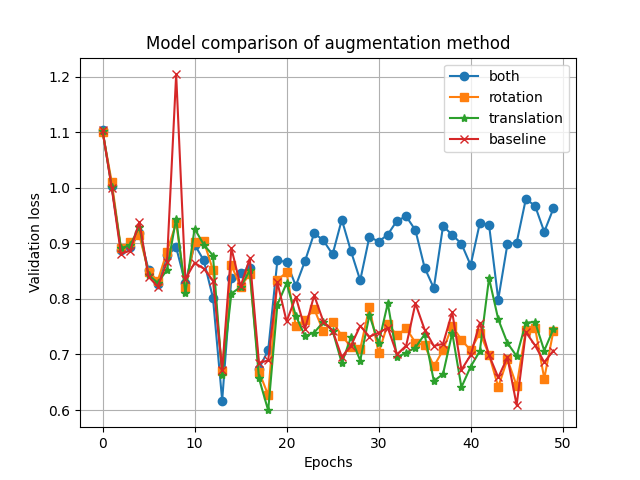
\includegraphics[width=\linewidth]{augmentation method_Validation loss.png}
    %     \caption{Augmentation method loss comparison}
    %     \label{aug_loss}
    % \end{minipage}
\end{figure}
\paragraph{}
At this point in the experiment process, the experiments will proceed without any augmentation, other options will be explored to address the data collection bias element.

% \subsection{Most effective spectral bands to use}
% \subsection{Image resizing methodology}
\section{Training experiments}
\subsection{Network Hyperparameters}
Given the complexity of an optimiser's performance and its interaction with the learning rate and batch size parameters, a comprehensive grid search experiment was performed to avoid a misleading evaluation of the parameters to follow.
% Full results of this grid search experiment can be found in the Annex. 

For simplicity, the same approach of only varying one parameter at a time, to ease interpretation, will be presented in the following subsections.

\subsection{Optimiser}
\paragraph{}
As introduced  in section \ref{optimiser}, there are several optimisers that could significantly affect the performance of the model. Even though \gls{SGD} seems to be the algorithm used by all the state-of-the-art segmentation models presented in section \ref{seg_nets}, the results of varying four different optimisers will be presented to see how the model is impacted by it.

\begin{figure}[hbt!]
    % \begin{minipage}[c]{0.45\linewidth}
    %     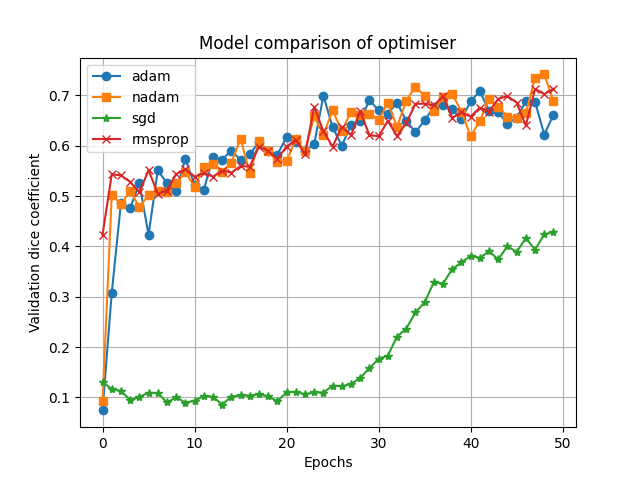
\includegraphics[width=\linewidth]{optimiser_Validation dice coefficient.png}
    %     \caption{Optimiser dice coefficient comparison}
    %     \label{opt_dice}
    %     \end{minipage}
    %     \hfill
    %     \begin{minipage}[c]{0.45\linewidth}
    \centering
    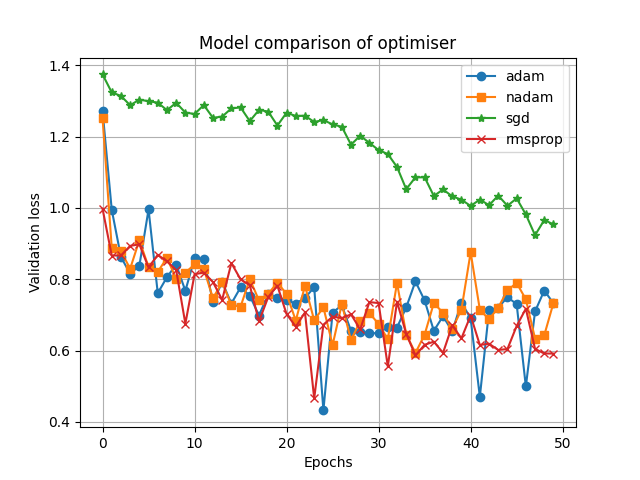
\includegraphics[width=0.75\linewidth]{optimiser_Validation loss.png}
    \caption{Optimiser Loss comparison}
    \label{opt_loss}
    % \end{minipage}
\end{figure}

\begin{table}[ht!] 
    \begin{center}
    \begin{tabular}{ccccccc} 
    \toprule
       & \multicolumn{3}{c}{Dice Coefficient}     & \multicolumn{3}{c}{Loss} \\
    Optimiser & Validation & Training & Test & Validation    & Training    & Test   \\ \midrule

    adam & 0.75 & 0.89 & 0.72 & 0.55 & 0.16 & 0.4  \\ nadam & 0.77 & 0.9 & 0.72 & 0.55 & 0.15 & 0.38  \\ sgd & 0.56 & 0.62 & 0.62 & 0.78 & 0.57 & 0.51  \\ \rowcolor{lightgray} rmsprop & 0.79 & 0.9 & 0.76 & 0.53 & 0.15 & 0.34  \\ 
    
    \bottomrule
    \end{tabular}
  \end{center} 
  \caption{Optimiser comparison of Dice Coefficient and Loss}\label{tab_opt}
\end{table}

Contradicting the literature, perhaps given the small dataset in this project compared with the millions of examples used to train state-of-the-art models, \gls{RMSProp} outperforms the other optimisers when it comes to loss minimisation as seen in Figure \ref{opt_loss}.

Figure \ref{opt_loss} shows similar validation loss coefficient between \gls{RMSProp}, \gls{NAdam} and \gls{Adam}, in order of minimisation performance, with \gls{SGD} lagging behind significantly, given the baseline learning rate of $0.0001$ and mini-batch size of $4$.

This may be due to the fact that the default parameters (apart from learning rate) of the Tensorflow implementation of all the optimisers are being used and need tuning for better performance and perhaps that \gls{Adam} is better used in problems with a lot of data and/or parameters. (\cite{kingma2017adam}) 

Given its performance, \gls{RMSProp} will be the optimiser of choice in the experiments to follow.
\subsection{Learning rate}
\paragraph{}
The Keras method "ReduceLROnPlateau" was applied, this involved reducing the learning rate by a factor of $10$, if there is no improvement in the validation set loss for $10$ epochs. This is enabled by the callback method that monitor loss and other metrics for each epoch.

The initial learning rate was chosen from $0.01$, $0.001$, $0.0001$, based on the literature introduced in section \ref{learning_rate} for this experiment, the results can be seen in Table \ref{tab_lr}.

\begin{table}[ht!] 
    \begin{center}
    \begin{tabular}{ccccccc} 
    \toprule
       & \multicolumn{3}{c}{Dice Coefficient}     & \multicolumn{3}{c}{Loss} \\
    Learning rate & Validation & Training & Test & Validation    & Training    & Test   \\ \midrule
    0.01 & 0.35 & 0.35 & 0.33 & 1.03 & 0.91 & 0.9  \\ 0.001 & 0.75 & 0.92 & 0.8 & 0.86 & 0.11 & 0.28  \\ \rowcolor{lightgray} 0.0001 & 0.79 & 0.9 & 0.76 & 0.53 & 0.15 & 0.34  \\
\bottomrule
    \end{tabular}
  \end{center} 
  \caption{Learning rate comparison of Dice Coefficient and Loss}\label{tab_lr}
\end{table}
\begin{figure}[hbt!]

\centering
    % \begin{minipage}[c]{0.45\linewidth}
    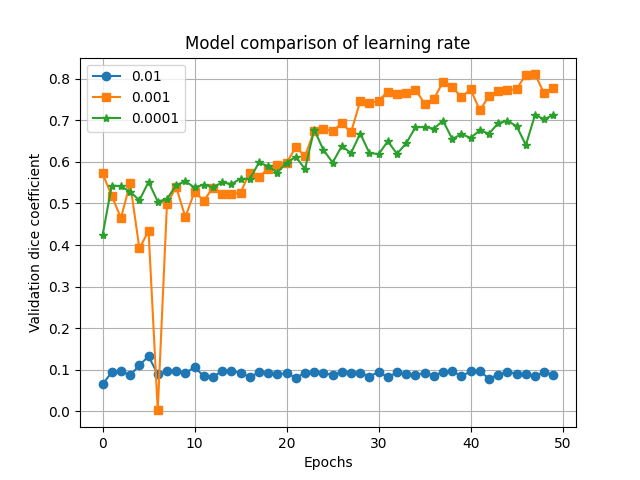
\includegraphics[width=0.75\linewidth]{learning rate_Validation dice coefficient.png}
    \caption{Learning rate Dice Coefficient comparison}
    \label{lr_dice}
    %     \end{minipage}
    %     \hfill
    %     \begin{minipage}[c]{0.45\linewidth}
    %     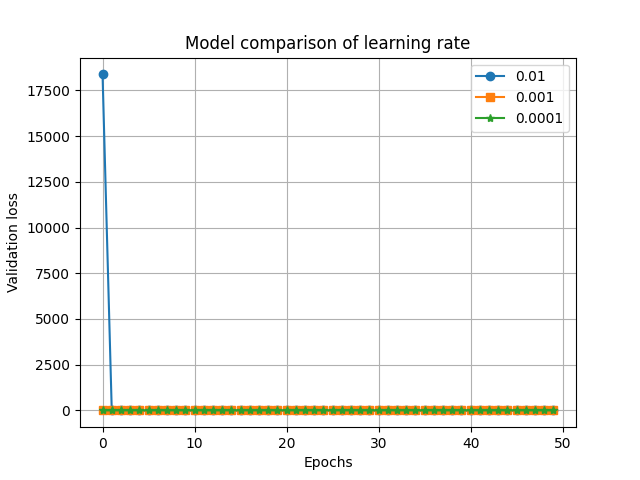
\includegraphics[width=\linewidth]{learning rate_Validation loss.png}
    %     \caption{Learning rate loss comparison}
    %     \label{lr_loss}
    % \end{minipage}
\end{figure}

Figure \ref{lr_dice} shows a big difference between the performance of $0.01$ learning rate and the other values, this could be due to the large learning rate overshooting the global or a local minimum and arriving at a suboptimal final set of weights.
In the grid search experiment, the initial learning rate of $0.01$ seemed to only perform well with the \gls{SGD} optimiser and vice versa, the \gls{SGD}  optimiser only performed well with the $0.01$ learning rate. This could be because the initital large learning rate allows SGD to do exploration of the search space early on and later on reducing through the "ReduceLROnPlateau" learning rate schedule allowing for the explotation of the search space in later epochs to get closer to the optimal loss.

The top learning rate for the RMSProp optimiser was $0.0001$, therefore this will be used for the experiments.

\subsection{Batch size}
\paragraph{}
Varying the mini-batch size has great implications in the convergence of the model, given its small labelled dataset, this project is working with smaller batch sizes than it is standard in the industry.

This is validated by the results of the experience, as it can be seen in Table \ref{tab_batch} the batch sizes that show the worst performance are the $2$  highest values of $16$ and $20$ mini-batch size. All the other values display a very close performance, with the best being a batch size of $1$.

\begin{table}[ht!] 
    \begin{center}
    \begin{tabular}{ccccccc} 
    \toprule
       & \multicolumn{3}{c}{Dice Coefficient}     & \multicolumn{3}{c}{Loss} \\
    Batch size & Validation & Training & Test & Validation    & Training    & Test   \\ \midrule
%\rowcolor{lightgray}
    \rowcolor{lightgray} 1 & 0.85 & 0.93 & 0.8 & 0.47 & 0.1 & 0.29  \\ 2 & 0.79 & 0.88 & 0.77 & 0.46 & 0.17 & 0.31  \\ 4 & 0.68 & 0.84 & 0.71 & 0.6 & 0.23 & 0.39  \\ 6 & 0.67 & 0.83 & 0.73 & 0.61 & 0.25 & 0.37  \\ 10 & 0.58 & 0.65 & 0.64 & 0.65 & 0.51 & 0.49  \\ 16 & 0.55 & 0.7 & 0.5 & 0.63 & 0.45 & 0.7  \\ 20 & 0.49 & 0.65 & 0.66 & 0.82 & 0.51 & 0.48  \\

    \bottomrule
    \end{tabular}
  \end{center} 
  \caption{Batch size comparison of Dice Coefficient and Loss}\label{tab_batch}
\end{table}

    % \begin{figure}[hbt!]
    %     \centering
    %     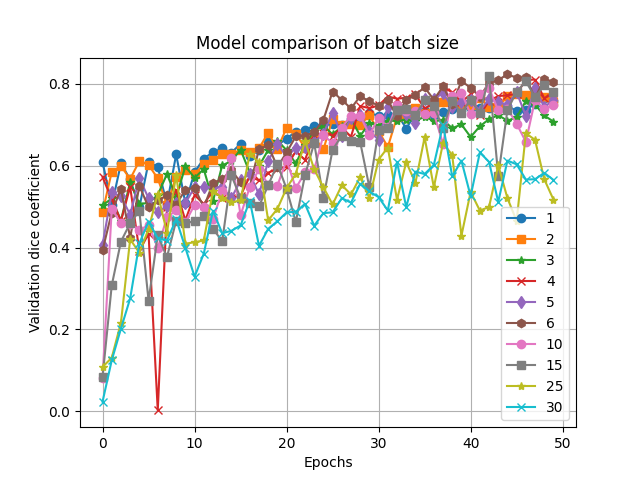
\includegraphics[width=0.9\textwidth]{batch size_Validation dice coefficient.png}
    %     \caption{Batch size dice coefficient comparison}
    %     \label{batch_dice}
    % \end{figure}



\subsection{Initialisation}
\paragraph{}
As presented in section \ref{initialisation}, "He" initialisation methods outperform the "Xavier" (glorot) initialisation method, according to the literature "He" initialisation works better mathematically by adressing the nonlinearities of the \gls{ReLU} activation function, which are also present in the \gls{ELU} activation function. 

The random normal initialiser has the same final performance as the "He" normal method in Table \ref{tab_init}, this results may have been due to a particularly good random weight initialisation, in order to assess it's validity it should be run several times to establish it's significance, however due to time and computational constraints this author did not investigate this further.

In a complete opposite way, using the random uniform initialisation function leads to a low stagnated validation dice coefficient, as can be seen from Figure \ref{init_dice}. This may be due to a bad initialisation, which lead to the backpropagation algorithm being unable to identify the right direction to transform the weights to optimise the cost function, which consequently stalls training.

\begin{table}[ht!] 
    \begin{center}
    \begin{tabular}{ccccccc} 
    \toprule
       & \multicolumn{3}{c}{Dice Coefficient}     & \multicolumn{3}{c}{Loss} \\
    Initialisation method & Validation & Training & Test & Validation    & Training    & Test   \\ \midrule
%\rowcolor{lightgray}
    \rowcolor{lightgray} he normal & 0.82 & 0.93 & 0.76 & 0.57 & 0.1 & 0.35  \\ he uniform & 0.8 & 0.92 & 0.77 & 0.65 & 0.11 & 0.34  \\ glorot normal & 0.79 & 0.87 & 0.71 & 0.47 & 0.19 & 0.4  \\ glorot uniform & 0.77 & 0.85 & 0.75 & 0.51 & 0.24 & 0.34  \\ random normal & 0.82 & 0.91 & 0.76 & 0.59 & 0.14 & 0.34  \\ random uniform & 0.69 & 0.72 & 0.67 & 0.64 & 0.45 & 0.45  \\
    \bottomrule
    \end{tabular}
  \end{center} 
  \caption{Initialisation method comparison of Dice Coefficient and Loss}\label{tab_init}
\end{table}

However, by looking at Figure \ref{init_dice} "He" Normal seems to be more stable and achieve a better performance at an earlier step than the Random Normal initialiser, therefore going forward the "He" Normal initialisation method will be used.

\begin{figure}[hbt!]
    % \begin{minipage}[c]{0.45\linewidth}
    \centering
    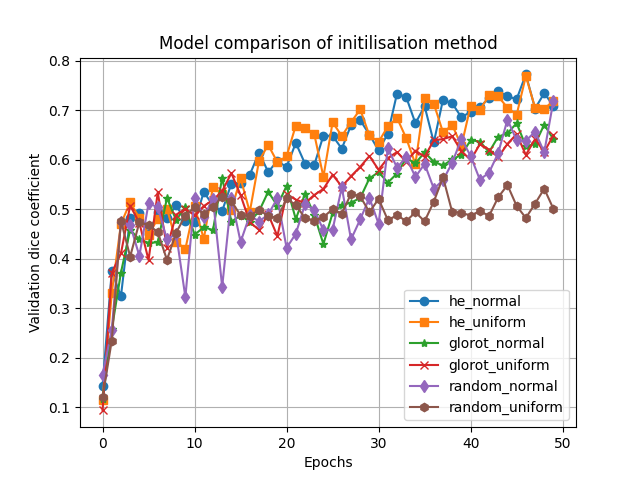
\includegraphics[width=0.75\linewidth]{initilisation method_Validation dice coefficient.png}
    \caption{Initialisation method Dice Coefficient comparison}
    \label{init_dice}
    %     \end{minipage}
    %     \hfill
    %     \begin{minipage}[c]{0.45\linewidth}
    %     \includegraphics[width=\linewidth]{init_evaluation_loss_elu.png}
    %     \caption{Initialisation method dice loss comparison}
    %     \label{init_loss}
    % \end{minipage}
\end{figure}    

From here on, "He" Normal initialisation will be used for the consequent experiments.

\subsection{Activation function}
\paragraph{}
The discussion of the advantages and disadvantages of different the different activation functions has been discussed in detail in section \ref{cnn_activation}.

From Figure \ref{loss_dice} \gls{ReLU} stands out since the validation loss completely stalls which indicates that the entire network has died, leading to unsuccessful convergence despite increasing the number of epochs. Dying \gls{ReLU} is a known phenomena with many explanations on how neurons become inactive always outputting $0$ for any given input. Lu et al. argue that symmetric probability distributions such as "He" initialisation for initialisation is a big cause of dying \gls{ReLU} and propose their own randomised asymmetric initialisation (\cite{Lu_2020}).

On the contrary, \gls{ELU} performs very well, having the highest Validation Dice coefficient, as can be seen from Table \ref{tab_act}. Since the constant value of $0$ for any negative input range is what causes dying \gls{ReLU},using one of its variations in this experiment avoids the problem associated with the zero-slope segment.

The \gls{SELU} function was also considered but as it is self normalising the \gls{NN} (\cite{klambauer2017selfnormalizing}) it deemed necessary yet another implementation, LeCun Normal initialisation and a special version of Dropout called Alpha Dropout, which this author did not perform at this point.

\begin{figure}[hbt!]
    % \begin{minipage}[c]{0.45\linewidth}
    \centering
    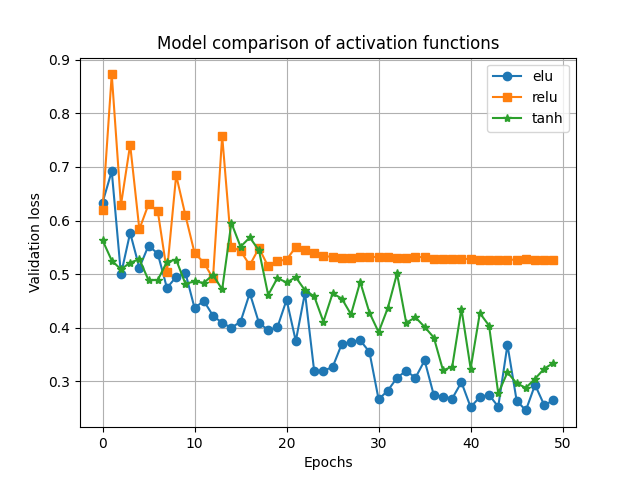
\includegraphics[width=0.75\textwidth]{activation functions_Validation loss.png}
    \caption{Activation function Loss comparison}
    \label{act_dice}
    %     \end{minipage}
    %     \hfill
    %     \begin{minipage}[c]{0.45\linewidth}
    %     \includegraphics[width=\linewidth]{act_evaluation_loss_uniform.png}
    %     \caption{Activation function loss comparison}
    %     \label{act_loss}
    % \end{minipage}
\end{figure}

\begin{table}[ht!]
    \begin{center}
    \begin{tabular}{ccccccc}
        \toprule
       & \multicolumn{3}{c}{Dice Coefficient}     & \multicolumn{3}{c}{Loss} \\
    Activation Function & Validation & Training & Test & Validation    & Training & Test   \\ 
    \rowcolor{lightgray} \gls{ELU} & 0.85 & 0.93 & 0.78 & 0.26 & 0.11 & 0.31  \\ \gls{ReLU} & 0.67 & 0.73 & 0.64 & 0.53 & 0.45 & 0.52  \\ tanh & 0.8 & 0.88 & 0.77 & 0.33 & 0.19 & 0.32  \\
                    \bottomrule
    \end{tabular}
    \caption{Activation function comparison of Dice Coefficient and Loss} \label{tab_act}
  \end{center}
\end{table}

\gls{ELU} proves to be the highest performing activation function, so it will remain being used in the following experiments.

\subsection{Loss Function} \label{loss_exp}
\paragraph{}
The chosen measure of performance for this project is the dice coefficient, an adequate loss function needs to be implemented in a way that minimising it, maximises the dice coefficient. To achieve this, the loss functions introduced in section \ref{loss_functions} were implemented in Python and compared to identify the best suited function for this project.

The implementation of the loss functions in Python under the Tensorflow Keras framework required a substantial amount of effort, as they were custom losses and required special attention to make sure matrix dimensions were correct for backpropagation to work and training to be successful. 

Figure \ref{loss_dice} shows that they are all successfully training the model as the chosen model scoring metric is showing an increasing trend as the number of epochs increase as would be expected if the gradient descent is working correctly.

\begin{figure}[hbt!]
    % \begin{minipage}[c]{0.45\linewidth}
    \centering
    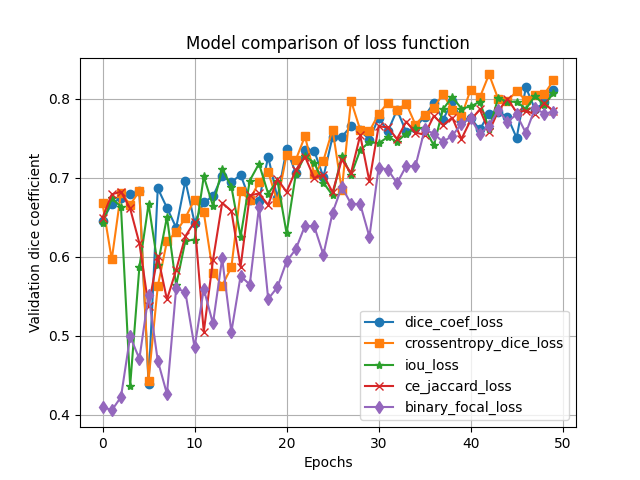
\includegraphics[width=0.75\linewidth]{loss function_Validation dice coefficient.png}
    \caption{Loss function Dice Coefficient comparison}
    \label{loss_dice}
        % \end{minipage}
    %     \hfill
    % \begin{minipage}[c]{0.45\linewidth}
    %     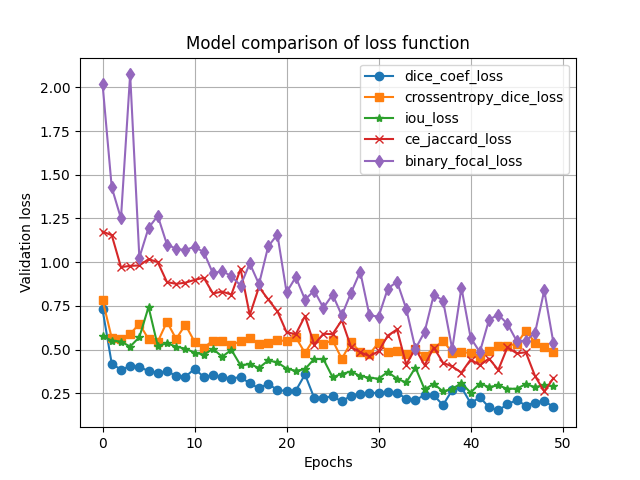
\includegraphics[width=\textwidth]{loss function_Validation loss.png}
    %     \caption{Loss function loss comparison}
    %     \label{loss_loss}
    % \end{minipage}
\end{figure}

\begin{table}[ht!] 
    \begin{center}
    \begin{tabular}{ccccccc} 
    \toprule
       & \multicolumn{3}{c}{Dice Coefficient}     & \multicolumn{3}{c}{Loss} \\
    Loss Function & Validation & Training & Test & Validation    & Training & Test   \\ 
    \midrule
    dice coef loss & 0.81 & 0.9 & 0.75 & 0.19 & 0.1 & 0.25  \\ \rowcolor{lightgray} \gls{CE} dice loss & 0.82 & 0.93 & 0.81 & 0.57 & 0.1 & 0.28  \\ iou loss & 0.81 & 0.91 & 0.71 & 0.29 & 0.15 & 0.45  \\ \gls{CE} jaccard loss & 0.78 & 0.93 & 0.8 & 1.06 & 0.18 & 0.51  \\ binary focal loss & 0.78 & 0.86 & 0.77 & 2.2 & 0.25 & 0.45  \\
    \bottomrule
    \end{tabular}
  \end{center} 
  \caption{Loss function comparison of Dice Coefficient and Loss}\label{tab_loss}
\end{table}

The best loss function is still the \gls{CE} dice loss, this could be because combining the two losses allows for some diversity, whilst still benefitting from the stability of \gls{CE}, so it will continue to be used in the following experiments.

% \subsection{Architecture Hyperparameters}
% \paragraph{Number of Filters}
% \paragraph{Kernel size and Stride of Conv}
% \paragraph{Kernel size and Stride of Pooling}
% \paragraph{Number of Layers}
% \paragraph{Dropout value}

\subsection{Preventing over-fitting} \label{regularisation_sec}
\subsubsection{\gls{ES}}
\paragraph{}
In the previous section the models ran for $50$ epochs without \gls{ES} implementation, given the experiments performed what is the impact of running a couple of the experiments applying \gls{ES} and how it affects the performance of the model.

The early stopping strategy consisted of monitoring the validation set loss for $15$ epochs (patience parameter) after which training will be stopped if there is no improvement (absolute change of less than $0$ (min delta parameter)) in the validation loss.

In order to perform this experiment an arbitrarily large number of epochs was set to $200$, \gls{ES} was triggered at $79$ epochs when validation loss did not improve from $0.24$, as can be seen from Figure \ref{es_loss} \gls{ES} was successful at preventing an overfitting situation, as the loss increased after epoch $79$.

\begin{figure}[hbt!]
    % \begin{minipage}[c]{0.45\linewidth}
    %     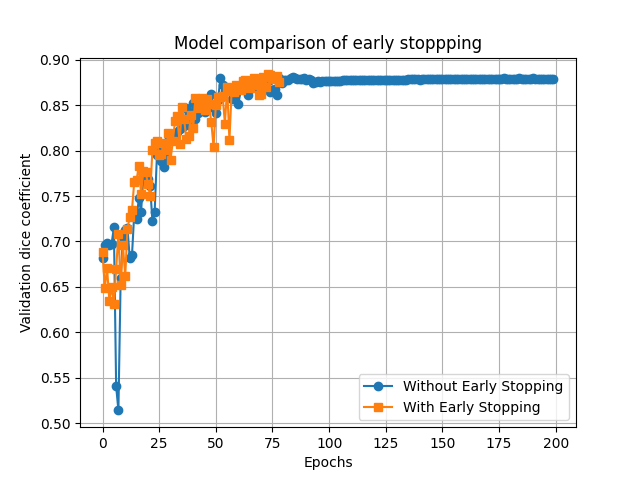
\includegraphics[width=\linewidth]{early stoppping_Validation dice coefficient.png}
    %     \caption{Loss function dice coefficient comparison of \gls{ES} usage}
    %     \label{es_dice}
    %     \end{minipage}
    %     \hfill
    % \begin{minipage}[c]{0.45\linewidth}
    \centering
    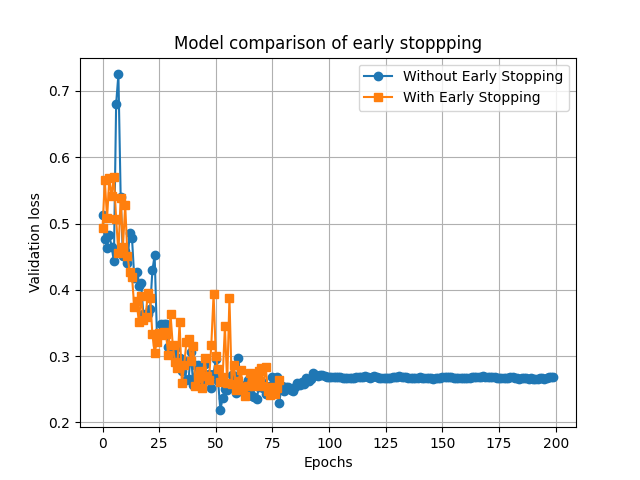
\includegraphics[width=0.75\textwidth]{early stoppping_Validation loss.png}
    \caption{\gls{ES} usage Loss comparison}
    \label{es_loss}
    % \end{minipage}
\end{figure}

\subsubsection{Dropout}
\paragraph{}
As part of the base network architecture introduced in section \ref{pixel_model}, Dropout has been implemented at different degrees starting at $0.1$ dropout rate and increasing by $0.1$ as one progresses deeper into the network.

As an experiment, the network with the same architecture with one change, all the dropout values introduced will be reduced to $0$, so there is no Dropout in the network.

\begin{figure}[hbt!]
    % \begin{minipage}[c]{0.45\linewidth}
    %     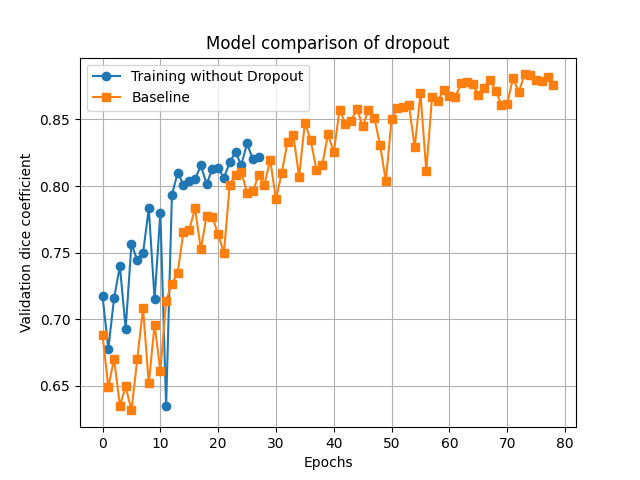
\includegraphics[width=\linewidth]{dropout_Validation dice coefficient.png}
    %     \caption{Loss function dice coefficient comparison of removal of Dropout}
    %     \label{dropout_dice}
    %     \end{minipage}
    %     \hfill
    % \begin{minipage}[c]{0.45\linewidth}
    \centering
    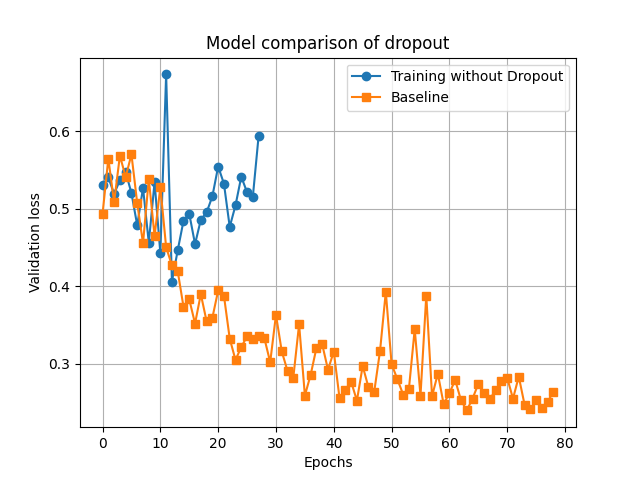
\includegraphics[width=0.75\textwidth]{dropout_Validation loss.png}
    \caption{Removal of Dropout Loss comparison}
    \label{dropout_loss}
    % \end{minipage}
\end{figure}

Without dropout in place the validation loss starts increasing drastically which triggers \gls{ES} much earlier, as we can see from Figure \ref{dropout_loss} this could be due to exploding gradients.

\section{Learnings from conducting experiments}
\paragraph{}
In summary, there are a few things that have been concluded from the experiments conducted with the \textit{\gls{GEE} data} and will motivate the decisions made for the section that follows where the model will be trained on the \textit{\gls{JP2} data} .

\begin{enumerate}
    \item{When there is a background and foreground class, where the foreground class represents the \gls{ROI}, in this case the \gls{RTS} pixels, it is important to adjust the patch size of the image as a way of reducing pixel imbalance between the negative more frequent background class and the positive more valuable foreground class. Depending on the size of the \gls{ROI} this has to be done taking into consideration that context around the \gls{ROI} is also valuable in its correct identification. For example in the context of this thesis reducing the patch size showed improvement until the $64$x$64$ patch size, but once it was further reduced to $32$x$32$ the performance was worst.}
    \item{The relationship between the learning rate hyperparameter and the optimiser is very strong, this was particularly evident with a higher learning rate of $0.1$, which incredibly benefitted the \gls{SGD} optimiser but drastically reduced the performance of the other optimisers, perhaps more experiments with the other parameters of optimisers and different learning rate schedules would be interesting, given more time.}
    \item{The relationship between mini-batch size and learning rate also seems to be very important, despite changing optimiser, it was observed through the grid search experiment that batch size of $1$ works better with $0.0001$ learning rate, whereas batch size of $10$ performs better with $0.001$ learning rate, this may be due to the fact that by seeing more data with a bigger batch size the model is less likely to overshoot a minimum and hence can tolerate a higher initial learning rate and vice-versa.}
    \item {The correct technical implementation of loss functions is challenging, specially when dealing with bespoke data ingested from GeoTiFF file format but essential for the successful training of the model.}
    \item {\gls{ES} is very effective in preventing overfitting.}
    \item {Dropout is very effective in preventing exploding gradients.}
\end{enumerate}
